%%%%%%%%%%%%%%%%%%%%%%%%%%%%%%%%%%%%%%%%%
%
% Space Physics
% Practical 2B
%
%%%%%%%%%%%%%%%%%%%%%%%%%%%%%%%%%%%%%%%%%

%----------------------------------------------------------------------------------------
%	DOCUMENT CONFIGURATIONS
%----------------------------------------------------------------------------------------

\documentclass{article}

\title{\textbf {Space Physics} \\ Practical 2B\\ Data Analysis} % Title
\def\authorivan{Ivan \v Sinkarenko}
\def\authoranu{Anuraj Rajendraprakash}
\author{\authorivan\\\authoranu}

\usepackage{graphicx}
\usepackage{fullpage}
\usepackage{url}

% load package with ``framed'' and ``numbered'' option.
\usepackage[framed,numbered,autolinebreaks,useliterate]{mcode}

\begin{document}

\maketitle % Insert the title, author and date

\centerline{Referee: Gabriella Stenberg}

\setlength\parindent{0pt} % Removes all indentation from paragraphs

\renewcommand{\labelenumi}{\alph{enumi}.} % Make numbering in the enumerate environment by letter rather than number
\clearpage

\tableofcontents

\listoffigures

\clearpage

%----------------------------------------------------------------------------------------
%	SECTION 1. Introduction
%----------------------------------------------------------------------------------------

    

%----------------------------------------------------------------------------------------
%	SECTION 2. Time Series Data
%----------------------------------------------------------------------------------------
\section{Time Series Data}

\subsection{Question 1}

\begin{figure}[htb]
\centering
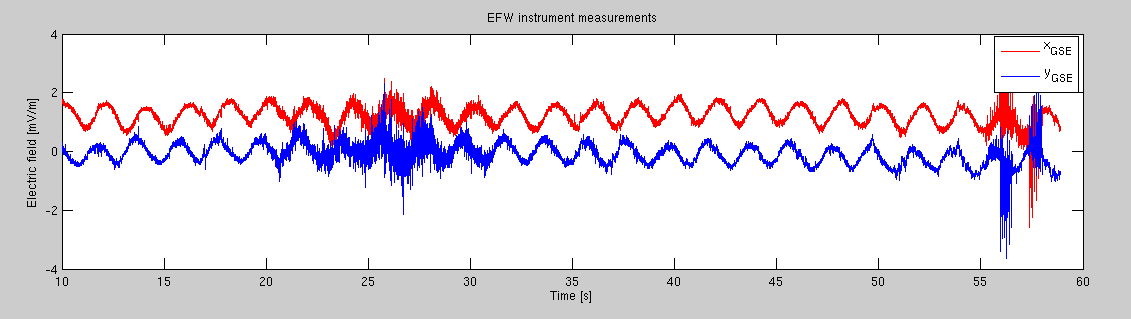
\includegraphics[width=\textwidth]{Figures/EFW_measurement.png}
\caption{EFW Measurement Data}
\label{fig:EFW}
\end{figure}

\begin{figure}[htb]
\centering
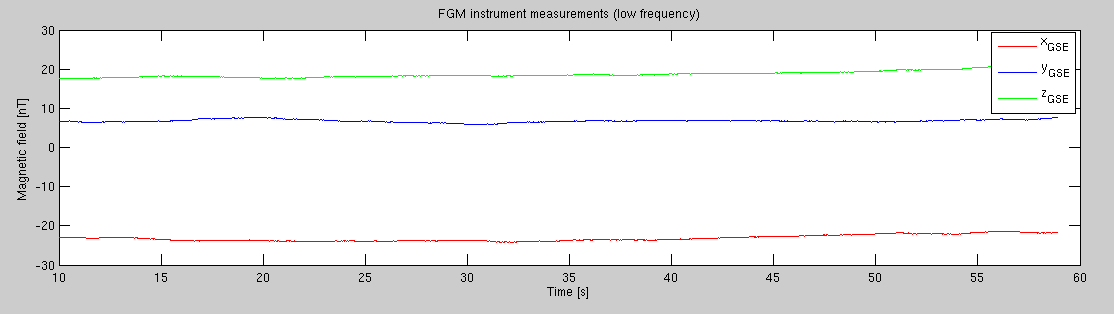
\includegraphics[width=\textwidth]{Figures/FGM_measurement.png}
\caption{FGM Measurement Data}
\label{fig:FGM}
\end{figure}

\begin{figure}[htb]
\centering
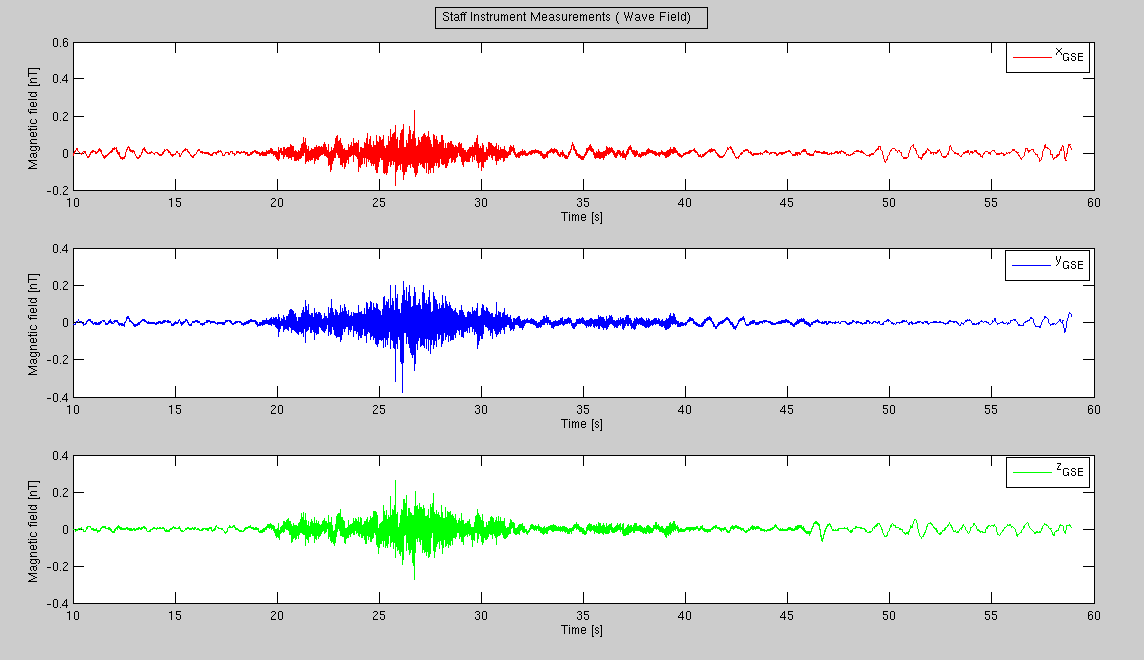
\includegraphics[width=\textwidth]{Figures/Staff_measurement.png}
\caption{Staff Instrument Measurement Data}
\label{fig:Staff}
\end{figure}



%----------------------------------------------------------------------------------------
%	SECTION 3. CONCLUSION
%----------------------------------------------------------------------------------------
%\newpage
\section{Conclusion}

This assignment has helped us get an idea of the design parameters of a phased array radar.
By varying the parameters that affect the design of a phased array antenna we observed how the radiation pattern varied. We learnt about the various techniques used for side lobe suppression in the radiation pattern. While doing this assignment we learnt about the trade off that has to be made between side lobe suppression and antenna gain in radars for MST weather applications. Finally we came to know about the parameters which are important while designing a practical phased array antenna.


%----------------------------------------------------------------------------------------
%	SECTION 4. REFERENCES
%----------------------------------------------------------------------------------------
\newpage
\begin{thebibliography}{9}

\bibitem{Enmark:2012a3}
Enmark A.  (2012).
\newblock {\em Assignment 3. Optimization of phased array antenna radiation pattern and array configuration}.
\newblock Lule\aa \ University of Technology, Kiruna, Sweden.

\bibitem{Skolnik:2001irs}
Skolnik M. ~I.  (2001).
\newblock {\em Introduction to Radar Systems}.
\newblock The McGraw-Hill Companies, Inc., New York, United States.

\bibitem{Rottger:2000ip}
R\"ottger J.  (2000).
\newblock {\em The Instrumental Principles of MST Radars and Incoherent Scatter Radars and The Configuration of Radar System Hardware}.
\newblock Max Planck Institut F\"ur Aeronomie, Katlenburg-Lindau, Germany.

\bibitem{Wiki:2012pa}
Wikipedia.org. (2012).
\newblock {\em Phased array}.
\newblock {\url{http://en.wikipedia.org/wiki/Phased_array}}.

\end{thebibliography}


%----------------------------------------------------------------------------------------
%	SECTION 5. Appendix 1
%----------------------------------------------------------------------------------------
\newpage
\section{Appendix 1. Matlab code}
%\lstinputlisting{assignment.m}

%----------------------------------------------------------------------------------------
%	SECTION 6. Confirmation
%----------------------------------------------------------------------------------------
\newpage
\section{Confirmation of Participation}

This is to confirm that the members of this team participated on the investigation of the required information to solve the assignment, generated their code to perform the calculation and discussed the results.\\
\vspace{2cm}
\newline
\line(1,0){200}\\
\authorivan\\
\vspace{2cm}
\newline
\line(1,0){200}\\
\authoranu\\


\end{document}